\runningheader{Oppgave h), frivillig}{}{Side \thepage\ av \numpages}

% ********************************************************
% oppgave h) 
% ********************************************************  
\item
  Kopier modellen fra g) og lag et nytt signal som
  \begin{equation}
    \label{eq:209}
    y(t) = 4{\cdot} u(t) {\cdot} t
  \end{equation}
  ved å bruke en {\sf  Gain}-blokk, en {\sf  Clock}-blokk og
  en {\sf  Product}-blokk.

  Utvid {\tt Scopet} til 6 innganger med 6 delfigurer for å vise $v_{1}(t)$,
  $v_{2}(t)$, $v_{3}(t)$,  $u(t)$, $t$ og $y(t)$.
    {\color{red}La simuleringstiden fortsatt være 25 sekund.  }
    Simuler modellen og ta med simuleringsresulatet
    i innleveringen din
    ved å bruke prosedyren på
     side~\pageref{page:prosedyre}.

  \begin{figure}[H]
    \centering
    \hspace*{0mm}\scalebox{0.55}{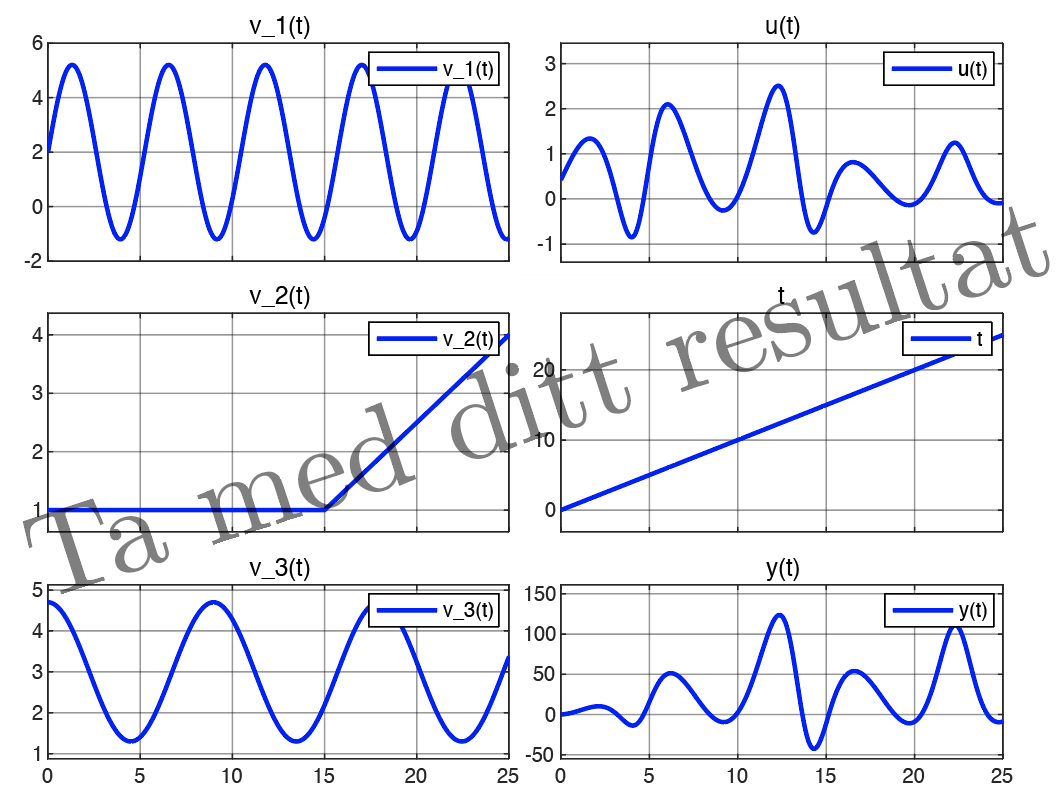
\includegraphics{fig_2h.png}}
    \caption{Simuleringsresultatet}
  \end{figure}

